\chapter{System Design}
\section{System Architecture}

\begin{figure}[h]\centering
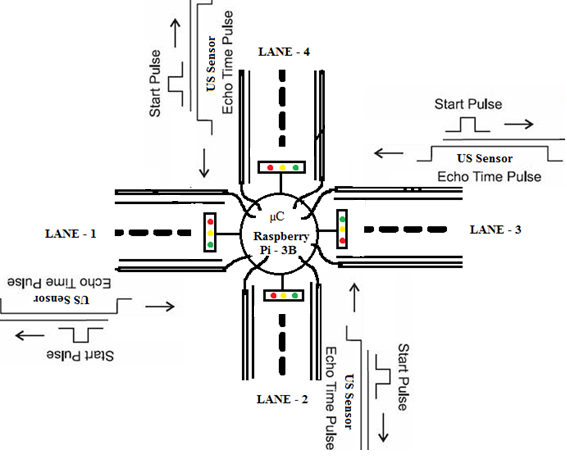
\includegraphics[width=5in]{./images/SystemArchitecture.png}
\caption{Architecture of Smart Traffic Control system using IOT}\label{design}
\end{figure}

\section{System Components}
\subsection{Ultrasonic Sensor}

The above shown HC-SR04 Ultrasonic (US) sensor is a 4-pin module, whose pin names are Vcc, Trigger, Echo and Ground respectively. It is used in many applications where measuring distance or sensing objects are required. The module has two eyes like projects in the front which forms the Ultrasonic transmitter and Receiver. The sensor works with the simple formula,

\begin{tabular}{lcr}
Distance &= Speed × Time & (3.1)\\
\end{tabular}
\begin{figure}[h]\centering
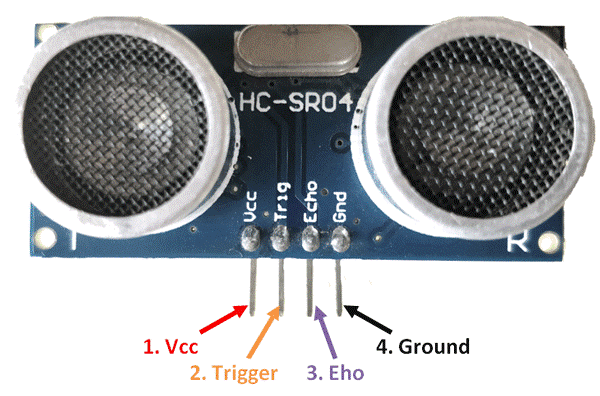
\includegraphics[width=2.5in]{./images/USsensor.png}
\caption{HC-SR04 Ultrasonic Sensor}\label{USsensor}
\end{figure}


The Ultrasonic transmitter transmits an ultrasonic wave, this wave travels in air and when it gets objected by any material it gets reflected back toward the sensor this reflected wave is observed by the Ultrasonic receiver module as shown in the figure \ref{USsensorWorking}

\begin{figure}[h]\centering
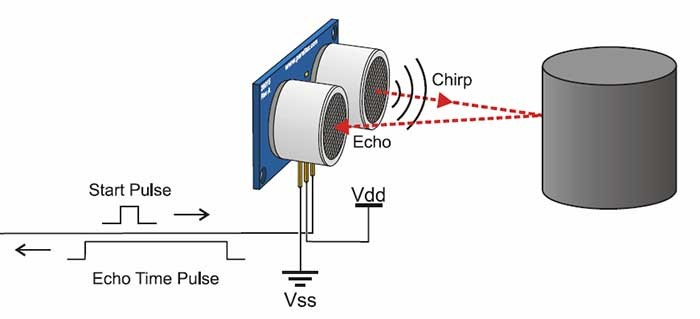
\includegraphics[width=5in]{./images/USsensorWorking.jpg}
\caption{HC-SR04 Ultrasonic Sensor Working}\label{USsensorWorking}
\end{figure}

Now, to calculate the distance using the above formula, we should know the Speed and time. Since the Ultrasonic wave is used, we know the universal speed of US wave at room conditions, which is 330m/s. The circuitry inbuilt on the module will calculate the time taken for the US wave to come back and turns on the echo pin high for that same particular amount of time, this way the time taken is known. Now the distance is calculated using the RPi microcontroller.

\pagebreak

\subsection{Raspberry Pi – 3B}

\begin{figure}[h]\centering
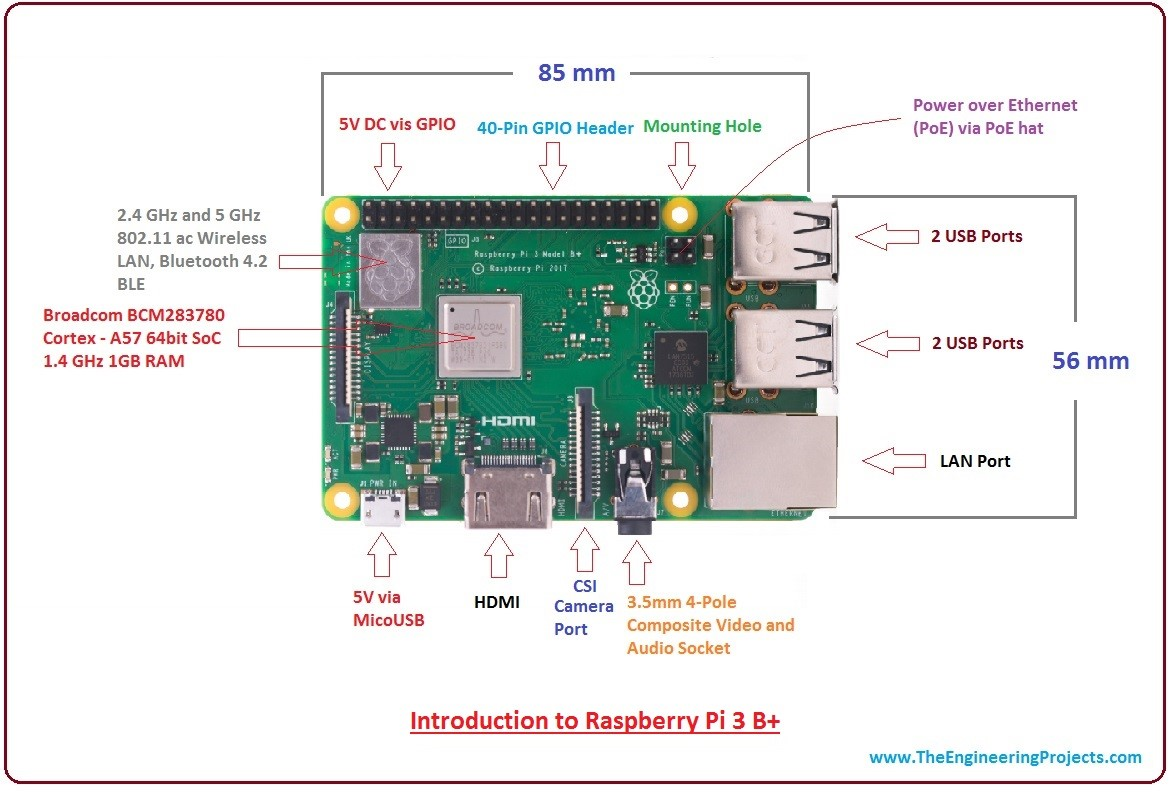
\includegraphics[width=5.5in]{./images/RaspberryPi.jpg}
\caption{Raspberry Pi - 3B}\label{RaspberryPi}
\end{figure}

Raspberry Pi – 3 is a development board in PI series. It can be considered as a single board computer that works on LINUX operating system. The board not only has tons of features it also has terrific processing speed making it suitable for advanced applications, who are interested in LINUX systems and IOT (Internet of Things).

All models feature a Broadcom system on a chip (SoC) with an integrated ARM-compatible central processing unit (CPU) and on-chip graphics processing unit (GPU).

The boards have one to five USB ports. For video output, HDMI and composite video are supported, with a standard 3.5 mm tip-ring-sleeve jack for audio output. Lower-level output is provided by a number of GPIO pins, which support common protocols like I²C. The B-models have an 8P8C Ethernet port and the Pi 3, Pi 4 and Pi Zero W have on-board Wi-Fi 802.11n and Bluetooth.

\pagebreak